\documentclass[a4paper,12pt]{ctexbook}
\usepackage[utf8]{inputenc}
\usepackage{graphicx}
\usepackage{amsmath}


\begin{document}

\begin{titlepage}
\begin{center}
\hspace{6cm}
\rule{\linewidth}{0.7mm}
{\heiti\zihao{0} 电磁场与电磁波\\[0.5cm]公式总结}\\[0.5cm]
\rule{\linewidth}{0.7mm}\\[2cm]

\begin{minipage}{0.4\textwidth}
	\begin{flushleft} \large
		\kaishu{编者:}\\
		\songti{朱 桐}
	\end{flushleft}
\end{minipage}
\begin{minipage}{0.4\textwidth}
	\begin{flushright} \large
		\kaishu{审校:} \\
		\songti{郑晓静}
	\end{flushright}
\end{minipage}
\vfill
\Large \today
\end{center}
\end{titlepage}

\frontmatter

\begin{center}
	$\heartsuit$\\[2.5cm]
	
	\LARGE \textit{For my Angel -- Miss. Zheng}\\[1cm]
	
	\begin{figure}[h]
		\centering
		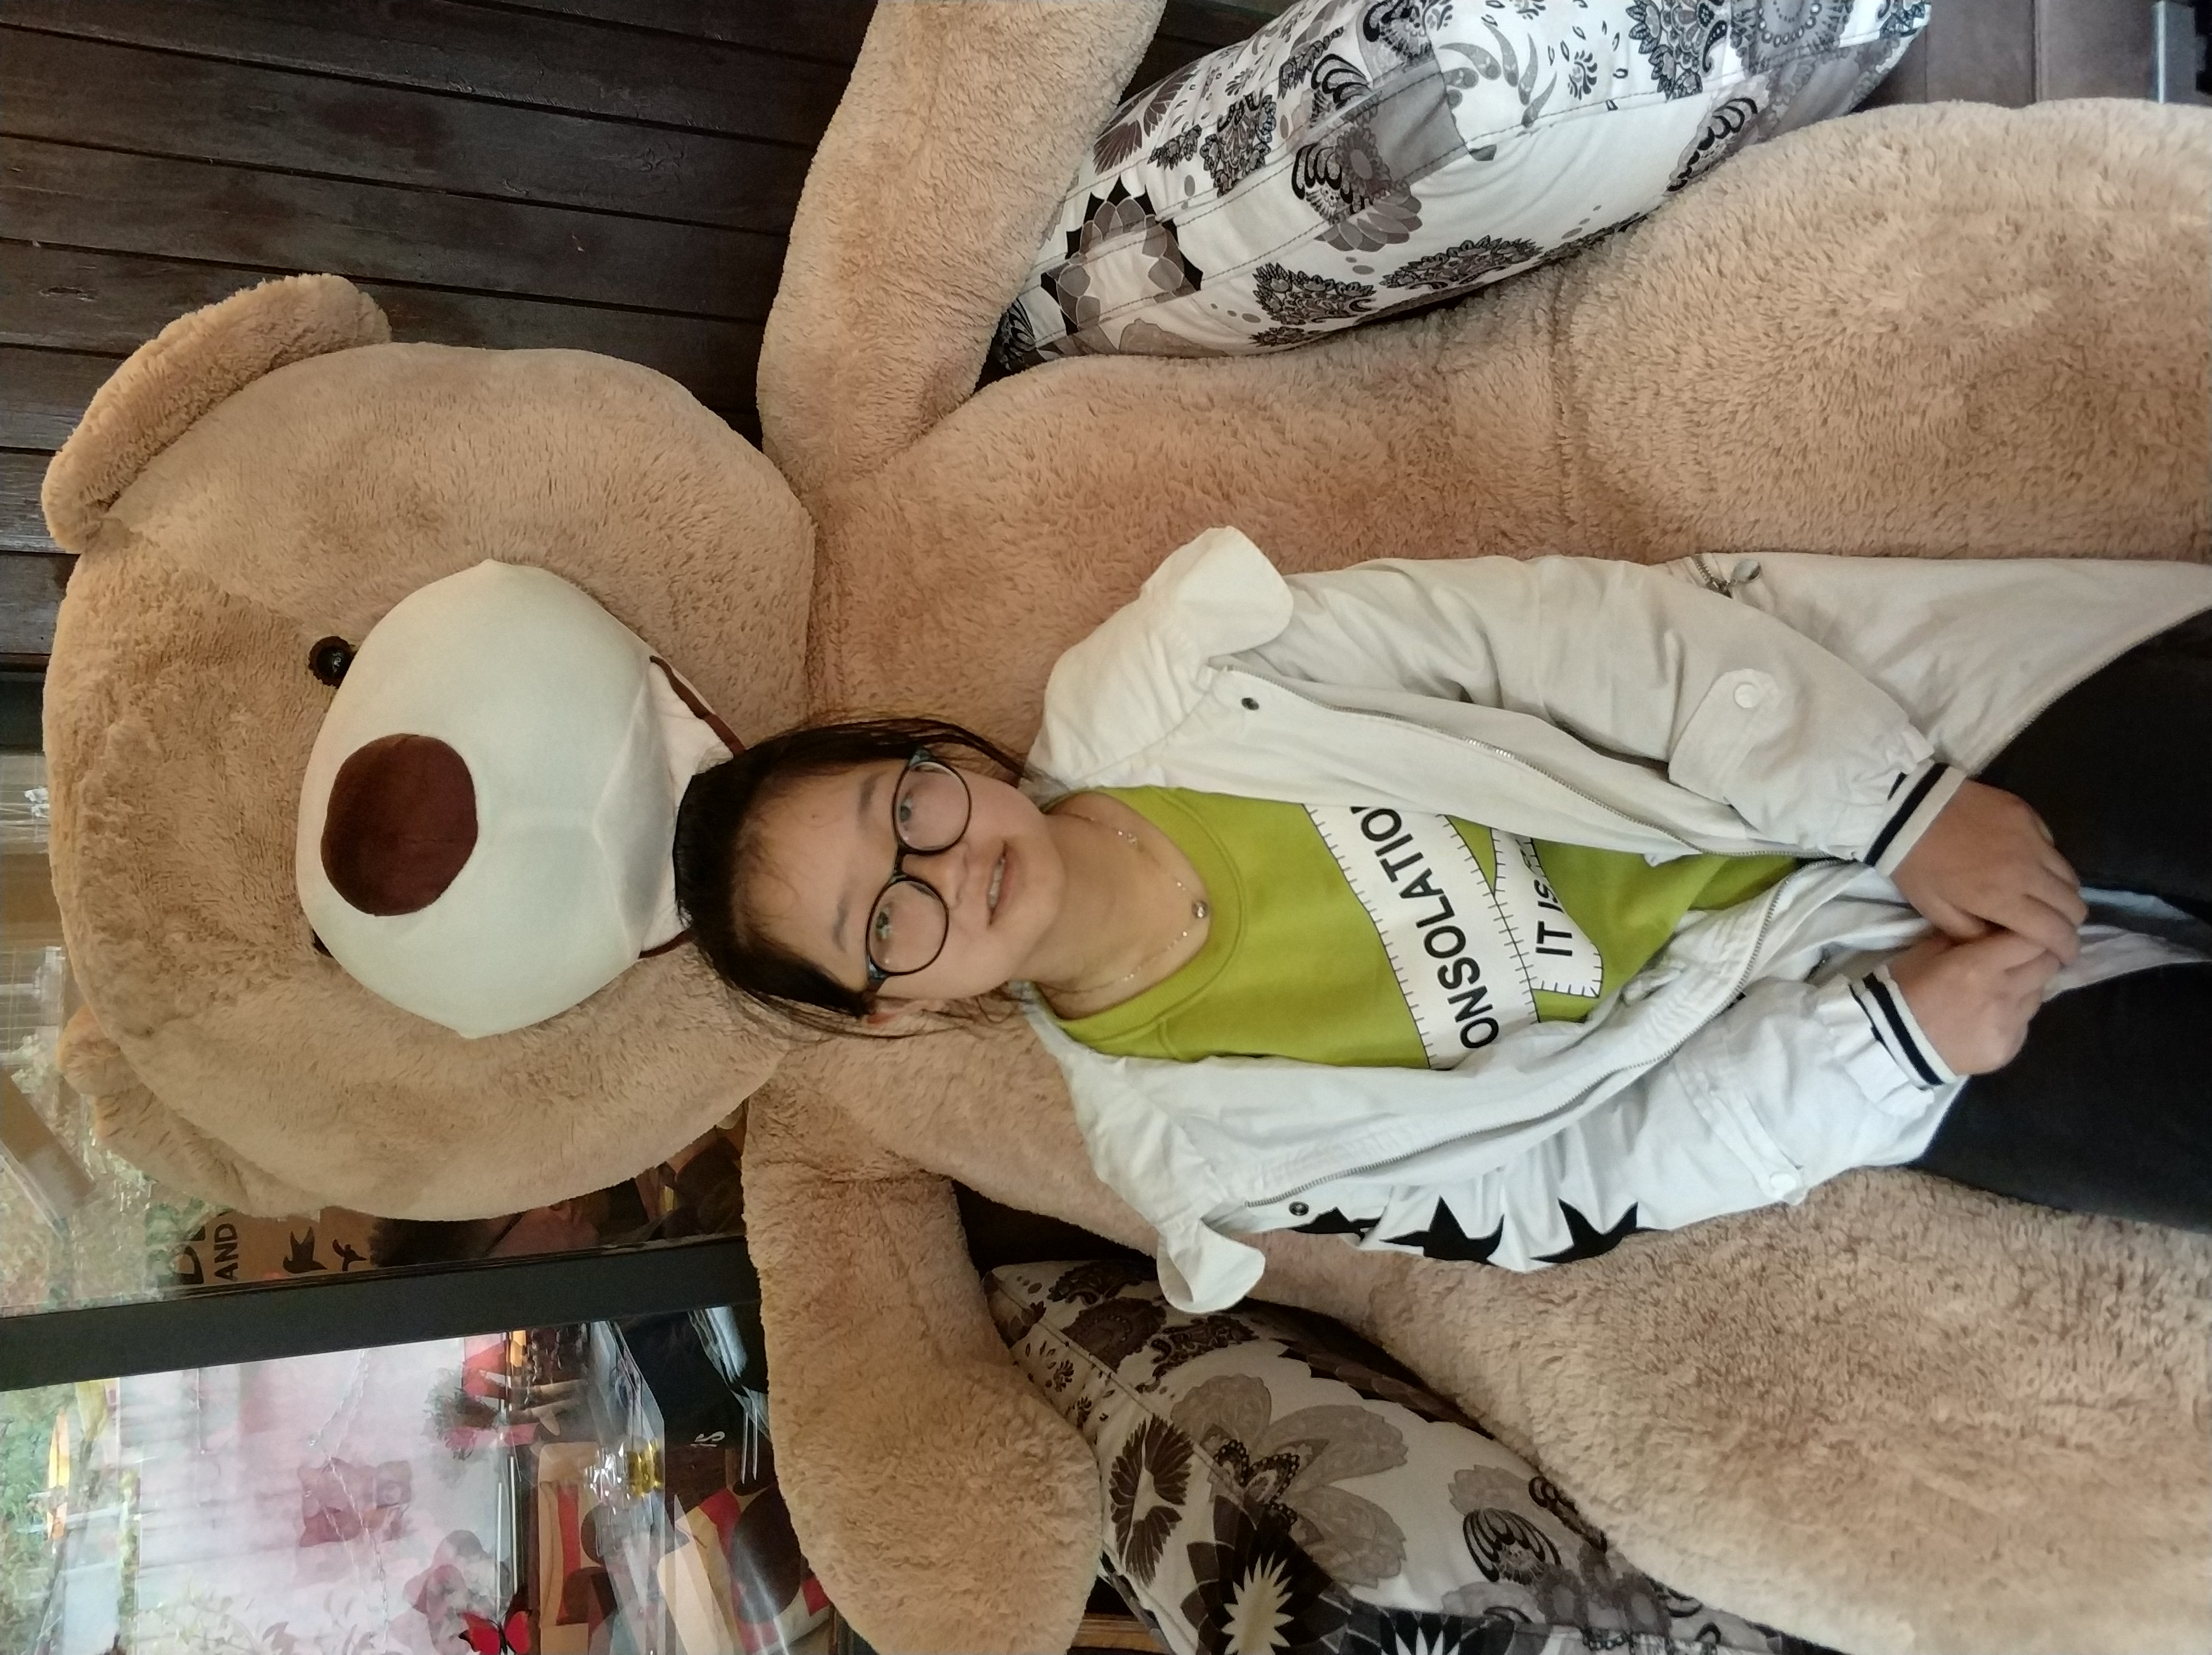
\includegraphics[keepaspectratio, height=10cm, angle=270]{pics/angel}
		\label{fig:angel}
	\end{figure}
	
\end{center}

\tableofcontents

\mainmatter
\chapter{矢量分析}

\section {矢量代数}
\begin{enumerate}
	\item 
		\begin{eqnarray}
		&\vec{A} \cdot \vec{B} = AB\cos\theta& \\
		&\vec{A}\bot\vec{B}\Rightarrow\vec{A}\cdot\vec{B}=0& \\
		&\vec{A}\parallel\vec{B}\Rightarrow\vec{A}\cdot\vec{B}=AB&
		\end{eqnarray}
	\item 
		\begin{eqnarray}
		&\vec A \times \vec B = {\vec e_n}AB\sin \theta& \\
		&\vec A \times \vec B = \left|\begin{array}{ccc}
									    \vec e_x & \vec e_y & \vec e_z  \\ 
										A_x & A_y & A_z  \\
										B_x & B_y & B_z
									\end{array} \right|& \\
		&\vec{A}\bot\vec{B} \Rightarrow \left| \vec{A} \times \vec{B} \right|= AB& \\
		&\vec{A}\parallel\vec{B} \Rightarrow \left| \vec{A} \times \vec{B} \right|= 0& \\
		&\vec{A}\cdot (\vec{B}\times \vec{C})=\vec{B}\cdot (\vec{C}\times \vec{A})=\vec{C}\cdot (\vec{A}\times \vec{B})& \\
		&\vec{A}\times (\vec{B}\times \vec{C})=(\vec{A}\cdot \vec{C})\vec{B}-(\vec{A}\cdot \vec{B})\cdot \vec{C}&
		\end{eqnarray}
		
\end{enumerate}
\section{三种常用的正交曲线坐标系}
\begin{enumerate}
	\item 直角坐标系 图\ref{fig:zhijiao}
	\item 圆柱坐标系 图\ref{fig:yuanzhu}
	\item 球坐标系	图\ref{fig:qiu}
		\begin{figure}
			\centering
			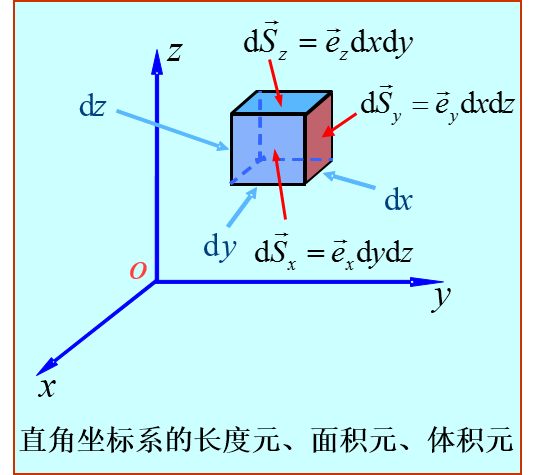
\includegraphics[keepaspectratio]{pics/直角坐标系}
			\caption{直角坐标系}
			\label{fig:zhijiao}
		\end{figure}
		\begin{figure}
			\centering
			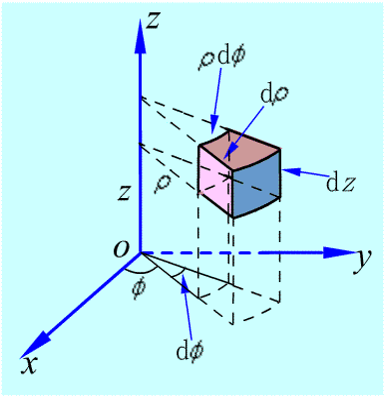
\includegraphics[keepaspectratio]{pics/圆柱坐标系}
			\caption{圆柱坐标系}
			\label{fig:yuanzhu}
		\end{figure}
		\begin{figure}
			\centering
			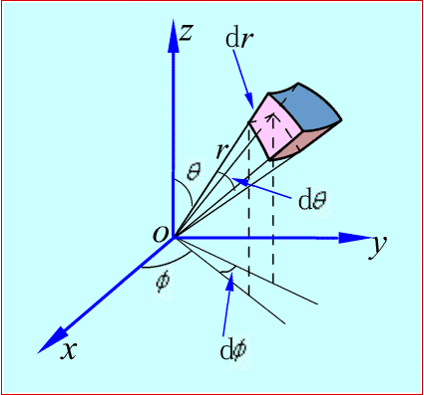
\includegraphics[keepaspectratio]{pics/球坐标系}
			\caption{球坐标系}
			\label{fig:qiu}
		\end{figure}
\end{enumerate}

\section{标量场的梯度}
\begin{enumerate}
	\item 方向导数
		\begin{eqnarray}
		&\frac{{\partial u}}{{\partial l}}\mathop |\nolimits_{{M_0}}  = \mathop {{\rm{lim}}}\limits_{\Delta l \to 0} \frac{{\Delta u}}{{\Delta l}} = \frac{{\partial u}}{{\partial x}}{\rm{cos}}\alpha  + \frac{{\partial u}}{{\partial y}}{\rm{cos}}\beta  + \frac{{\partial u}}{{\partial z}}{\rm{cos}}\gamma&
		\end{eqnarray}
	\item 梯度
		\begin{eqnarray}
		&\nabla u = {\vec e_x}\frac{{\partial u}}{{\partial x}} + {\vec e_y}\frac{{\partial u}}{{\partial y}} + {\vec e_z}\frac{{\partial u}}{{\partial z}}&
		\end{eqnarray}
\end{enumerate}

\section{矢量场的通量与散度}
\begin{enumerate}
	\item 通量
		\begin{eqnarray}
		&\psi  = \int {{\rm{d}}\psi  = } \int_S {\vec F \cdot {\rm{d}}\vec S}  = \int_S {\vec F \cdot {{\vec e}_n}{\rm{d}}S}&
		\end{eqnarray}
	\item 散度
		\begin{eqnarray}
		&\nabla  \cdot \vec F(x,y,z) = \mathop {\lim }\limits_{\Delta V \to 0} \frac{{\oint_S {\vec F(x,y,z) \cdot {\rm{d}}\vec S} }}{{\Delta V}}& \\
		&\nabla  \cdot \vec F = \frac{{\partial {F_x}}}{{\partial x}} + \frac{{\partial {F_y}}}{{\partial y}} + \frac{{\partial {F_z}}}{{\partial z}}&
		\end{eqnarray}
\end{enumerate}

\section{矢量场的环流和旋度}
\begin{enumerate}
	\item 环流
		\begin{eqnarray}
		&\Gamma  = \oint_C {\vec F(x,y,z) \cdot {\rm{d}}\vec l}	&
		\end{eqnarray}
	\item 环流面密度
		\begin{eqnarray}
		&{\rm{ro}}{{\rm{t}}_n}\vec F = \lim\limits_{\Delta S \to 0} \frac{1}{{\Delta S}}\oint_C {\vec F \cdot {\rm{d}}\vec l}	&
		\end{eqnarray}
	\item 旋度
		\begin{eqnarray*}
		&&{\rm{ro}}{{\rm{t}}_n}\vec F = {\vec e_n} \cdot \nabla  \times \vec F \\
		\nabla  \times \vec F&=&{\vec e_n}{[{\rm{ro}}{{\rm{t}}_n}\vec F]_{\max }} \\
		&=&{{\vec e}_x}\left( {{{\partial {F_z}} \over {\partial y}} - {{\partial {F_y}} \over {\partial z}}} \right) + {{\vec e}_y}\left( {{{\partial {F_x}} \over {\partial z}} - {{\partial {F_z}} \over {\partial x}}} \right) + {{\vec e}_z}\left( {{{\partial {F_y}} \over {\partial x}} - {{\partial {F_x}} \over {\partial y}}} \right) \\
		&=&\left| \begin{array}{ccc}
					{{{\vec e}_x}} & {{{\vec e}_y}} & {{{\vec e}_z}}  \\
					{{\partial  \over {\partial x}}} & {{\partial  \over {\partial y}}} & {{\partial  \over {\partial z}}} \\
					{{F_x}} & {{F_y}} & {{F_z}} 
					\end{array} \right|
		\end{eqnarray*}
	\item  两个恒等式
		\begin{eqnarray}
		&\nabla  \cdot (\nabla  \times \vec F) \equiv 0& \\
		&\nabla  \times (\nabla u) \equiv 0&
		\end{eqnarray}
	\item Stocks 定理
		\begin{eqnarray}
		&\oint_{{\kern 1pt} C} {{\kern 1pt} \vec F \cdot {\rm{d}}\vec l}  = \int_{{\kern 1pt} S} {{\kern 1pt} \nabla  \times \vec F \cdot {\rm{d}}\vec S}&
		\end{eqnarray}
\end{enumerate}

\section{拉普拉斯运算与格林定理}
\begin{enumerate}
	\item 格林定理(第一条是第一定理,后两条是第二定理)
	\begin{eqnarray}
	&\int_{V} (\nabla \Psi  \cdot \nabla \Phi  + \Psi {\nabla ^2}\Phi ){\rm{d}}V}  = \oint_{S} {(\Psi \nabla \Phi ) \cdot {\rm{d}}\vec S & \\
	&\int_{V} (\Psi {\nabla ^2}\Phi  - \Phi {\nabla ^2}\Psi ){\rm{d}}V}  = \oint_{S} {(\Psi \nabla \Phi  - \Phi \nabla \Psi ) \cdot {\rm{d}}\vec S& \\
	&\int_{V} (\Psi {\nabla ^2}\Phi  - \Phi {\nabla ^2}\Psi ){\rm{d}}V}  = \oint_{S} {(\Psi {{\partial \Phi } \over {\partial n}} - \Phi {{\partial \Psi } \over {\partial n}}){\rm{d}}S&
	\end{eqnarray}
\end{enumerate}

\section{亥姆霍兹定理}
\begin{enumerate}
	\item 亥姆霍兹定理
	\begin{eqnarray}
	&\vec F(\vec r) =  - \nabla u(\vec r) + \nabla  \times \vec A(\vec r)& \\
	&u(\vec r) = {1 \over {4{\rm{\pi }}}}\int_{{\kern 1pt} V} {{{\nabla ' \cdot \vec F(\vec r')} \over {\left| {\vec r - \vec r'} \right|}}} {\rm{d}}V'& \\
	&\vec A(\vec r) = {1 \over {4{\rm{\pi }}}}\int_{{\kern 1pt} V} {{{\nabla ' \times \vec F(\vec r')} \over {\left| {\vec r - \vec r'} \right|}}{\rm{d}}V'} &
	\end{eqnarray}
\end{enumerate}

\chapter{电磁场的基本规律}

\section{电子电荷值}
$$ e = 1.60219933 \times 10^{-19} \quad C $$

\section{电荷密度}

\subsection*{电荷体密度}
$$ \rho(\vec r) = \lim\limits_{\Delta V \to 0} \frac{\Delta q(\vec{r})}{\Delta V} = \frac{\mathrm{d}q(\vec{r})}{\mathrm{d}V} \quad C/m^3$$
反过来求电荷:
$$ q = \int_V \rho(\vec{r}) \mathrm{d}V $$

\subsection*{电荷面密度}
$$ \rho(\vec r) = \lim\limits_{\Delta S \to 0} \frac{\Delta q(\vec{r})}{\Delta S} = \frac{\mathrm{d}q(\vec{r})}{\mathrm{d}S} \quad C/m^2$$
$$ q = \int_S \rho_S(\vec{r}) \mathrm{d}S $$

\subsection*{电荷线密度}
$$ \rho(\vec r) = \lim\limits_{\Delta l \to 0} \frac{\Delta q(\vec{r})}{\Delta l} = \frac{\mathrm{d}q(\vec{r})}{\mathrm{d}l} \quad C/m$$
$$ q = \int_S \rho_S(\vec{r}) \mathrm{d}l $$

\subsection*{点电荷密度}
$$ \rho(\vec{r}) = q \cdot \delta(\vec{r} - \vec{r}') $$
其中,带“$'$”的是源点,不带的是场点。

\section{电流}
$$ i = \lim\limits_{\Delta t \to 0} \frac{\Delta q}{\Delta t} = \frac{\mathrm{d}q}{\mathrm{d}t} \quad A$$
电流方向为正电荷流动方向。不随时间变化的电流称为恒定电流:“$I$”。

\subsection*{体电流}
电流密度矢量:
$$ \vec{J} = \vec{e_n} \lim\limits_{\Delta S \to 0} \frac{\Delta i}{\Delta S} = \vec{e_n} \cdot \frac{\mathrm{d}i}{\mathrm{d}S} \quad A/m^2 $$
流过任意曲面的电流:
$$ i = \int_S\vec{J}\cdot\mathrm{d}\vec{S} $$

\subsection*{面电流}
电流密度矢量:
$$ \vec{J_S} = \vec{e_t} \lim\limits_{\Delta l \to 0} \frac{\Delta i}{\Delta l} = \vec{e_t} \cdot \frac{\mathrm{d}i}{\mathrm{d}l} \quad A/m $$
通过薄导体层上任意有向曲线$\vec{l}$的电流为:
$$ i = \int \vec{J} \cdot \left(\vec{e_n} \times \mathrm{d}\vec{l}\ \right)$$
其中,$\vec{e_n}$为平面法线方向,$\vec{e_t}$为有向曲线方向。

\subsection*{线电流}
长度元$\mathrm{d}l$;电流元:$I\mathrm{d}l$。

\subsection*{电流连续性方程}
流出闭曲面的电流等于体积$V$内单位时间所减少的电荷量。
积分式(总电荷增加率的负值):
$$ I = \oint_S \vec{J} \cdot \mathrm{d}\vec{S} = -\frac{\mathrm{d}q}{\mathrm{d}t} = -\frac{\mathrm{d}}{\mathrm{d}t} \int_V \rho \mathrm{d}V $$
微分式(电荷密度增加率):
$$ \nabla \cdot \vec{J} = -\frac{\partial \rho}{\partial t} $$
恒定电流的连续性方程:
$$ \frac{\partial \rho}{\partial t} = 0 \Rightarrow \nabla \cdot \vec{J} = 0,\quad \oint_S \vec{J} \cdot \mathrm{d}\vec{S} = 0 $$
恒定电流是无源场,电流线是连续的闭合曲线,既无起点也无终点。

\subsection*{传导电流密度}
$$ \vec{J} = \rho\vec{v} $$

\section{库仑定律(Coulomb)}
真空中静止点电荷$q_1$对$q_2$的作用力:
$${\vec F_{12}} = {\vec e_R}{{{q_1}{q_2}} \over {4{\rm{\pi }}{\varepsilon _0}R_{12}^2}} = {{{q_1}{q_2}{{\vec R}_{12}}} \over {4{\rm{\pi }}{\varepsilon _0}R_{12}^3}}$$
(自由空间中)$\varepsilon_0$:真空中的介电常数,$\varepsilon_0 \approx \frac{1}{36\pi}\times10^{-19}\approx8.85\times10^{-12}\quad F/m$

\section{电场强度}
$$\vec E(\vec r) = \mathop {{\rm{lim}}}\limits_{{q_0} \to 0} {{\vec F(\vec r)} \over {{q_0}}}$$
${q_0}$为试验电荷。真空中静止点电荷$q$激发的电场为:
$$\vec E(\vec r) = {{q\vec R} \over {4{\rm{\pi }}{\varepsilon _0}{R^3}}} \quad(\vec R = \vec r - \vec r')$$

体密度为$\rho(\vec{r})$的体分布电荷产生的电场强度:
\begin{eqnarray*}
	\vec E(\vec r) &=& \sum\limits_i {{{\rho ({{\vec r'}_i}){\rm{\Delta }}{{V'}_i}{{\vec R}_i}} \over {4{\rm{\pi }}{\varepsilon _0}R_i^3}}} \\
	&=&{1 \over {4{\rm{\pi }}{\varepsilon _0}}}\int_{{\kern 1pt} V} {{\kern 1pt} {{\rho (\vec r')\vec R} \over {{R^3}}}{\rm{d}}V'}
\end{eqnarray*}

面密度为$\rho_S(\vec{r})$的面分布电荷的电场强度:
$$\vec E(r') = {1 \over {4{\rm{\pi }}{\varepsilon _0}}}\int_{{\kern 1pt} S} {{\kern 1pt} {{{\rho _S}(\vec r')\vec R} \over {{R^3}}}{\rm{d}}S'} $$


线密度为$\rho_l(\vec{r})$的线分布电荷的电场强度:
$$\vec E(r') = {1 \over {4{\rm{\pi }}{\varepsilon _0}}}\int_{{\kern 1pt} C} {{\kern 1pt} {{{\rho _l}(\vec r')\vec R} \over {{R^3}}}{\rm{d}}l'} $$

\section{静电场}
\subsection*{静电场散度与高斯定理}
静电场散度:

微分形式:$$\nabla  \cdot \vec E{\rm{(}}\vec r{\rm{)}} = {{\rho {\rm{(}}\vec r{\rm{)}}} \over {{\varepsilon _0}}}$$

积分形式(高斯定理):$$\oint_{{\kern 1pt} S} {\vec E{\rm{(}}\vec r{\rm{)}} \cdot {\rm{d}}\vec S}  = {1 \over {{\varepsilon _0}}}\int_{{\kern 1pt} V} {\rho {\rm{(}}\vec r{\rm{)d}}V} $$

静电场是有源场。

\subsection*{静电场旋度与环路定理}
静电场旋度:
微分:$$\nabla  \times \vec E{\rm{(}}\vec r{\rm{)}} = 0$$

积分(环路定理):$$\oint_{{\kern 1pt} C} {\vec E{\rm{(}}\vec r{\rm{)}} \cdot {\rm{d}}\vec l}  = 0$$

静电场是无旋场(保守场),电场力做功与路径无关。


\section{安培力定律}
真空中载流回路$C_1$对载流回路$C_2$的作用力:
$${\vec F_{12}} = {{{\mu _0}} \over {4{\rm{\pi }}\,}}\oint_{{\kern 1pt} {C_2}} {\oint_{{\kern 1pt} {C_1}} {{{{I_2}{\rm{d}}{{\vec l}_2} \times ({I_1}{\rm{d}}{{\vec l}_1} \times {{\vec R}_{12}})} \over {R_{12}^3}}} } $$

$${\vec F_{12}} = \oint_{{\kern 1pt} {C_2}} {{I_2}{\rm{d}}{{\vec l}_2} \times ({{{\mu _0}} \over {4{\rm{\pi }}}}\oint_{{\kern 1pt} {C_1}} {{{{I_1}{\rm{d}}{{\vec l}_1} \times {{\vec R}_{12}}} \over {R_{12}^3}})} }  = \oint_{{\kern 1pt} {C_2}} {{I_2}{\rm{d}}{{\vec l}_2} \times {{\vec B}_1}({{\vec r}_2})} $$

其中,${\vec B_1}({\vec r_2}) = {{{\mu _0}} \over {4{\rm{\pi }}}}\oint_{{\kern 1pt} {C_1}} {{{{I_1}{\rm{d}}{{\vec l}_1} \times {{\vec R}_{12}}} \over {R_{12}^3}}} $为电流$I_1$在电流元$I_2\mathrm{d}\vec{l}_2$处产生的磁感应强度。

\section{磁感应强度}
\subsection*{任意电流回路$C$产生的磁感应强度}
$$\vec B(\vec r) = {{{\mu _0}} \over {4{\rm{\pi }}}}\oint_{{\kern 1pt} C} {{{I{\rm{d}}\vec l' \times (\vec r - \vec r')} \over {{{\left| {\vec r - \vec r'} \right|}^3}}}}  = {{{\mu _0}} \over {4{\rm{\pi }}}}\oint_{{\kern 1pt} C} {{{I{\rm{d}}\vec l' \times \vec R} \over {{R^3}}}} $$
电流元$I\mathrm{d}\vec{l}'$产生的磁感应强度

$${\rm{d}}\vec B(\vec r) = {{{\mu _0}} \over {4{\rm{\pi }}}}{{I{\rm{d}}\vec l' \times (\vec r - \vec r')} \over {{{\left| {\vec r - \vec r'} \right|}^3}}}$$

\subsection*{体电流激发的磁场}
$$\vec B(\vec r) = {{{\mu _0}} \over {4{\rm{\pi }}}}\int_{{\kern 1pt} V} {{{J{\rm{(}}\vec r') \times \vec R} \over {{R^3}}}{\kern 1pt} } {\rm{d}}V'$$

\subsection*{面电流激发的磁场}
$$\vec B(\vec r) = {{{\mu _0}} \over {4{\rm{\pi }}}}\int_{{\kern 1pt} S} {{{{J_S}{\rm{(}}\vec r') \times \vec R} \over {{R^3}}}{\kern 1pt} } {\rm{d}}S'$$

\section{恒定磁场的散度和旋度}
恒定磁场的散度与磁通连续性原理:
恒定场散度:$$\nabla \cdot \vec{B}(\vec{r})=0$$

磁通连续性原理:$$\oint_{{\kern 1pt} S} {\vec B(\vec r) \cdot {\rm{d}}\vec S}  = 0$$

恒定磁场是无源场,磁感应线是无起点和终点的闭合曲线。
恒定磁场的旋度与安培环路定理:
恒定磁场的旋度(微分形式):$$\nabla \times \vec{B}(\vec{r}) = \mu_0\vec{J}(\vec{r})$$

安培环路定理(积分形式):$$\oint_C\vec{B}(\vec{r}) \cdot \mathrm{d} \vec{l}  = \mu_0\int_{S} \vec{J}(\vec r) \cdot \mathrm{d} \vec S  = \mu_0I$$

恒定磁场是有旋场,是非保守场、电流是磁场的旋涡源。

\section{极化强度矢量$\vec{P}\quad(C/m^2)$}
介质极化程度:$$\vec P=\mathop {{\rm{lim}}}\limits_{\Delta V \to 0} {{\sum {{{\vec p}_i}} } \over {\Delta V}} = n\vec p=\chi_e\varepsilon_0\vec{E}$$

其中,$\vec{p}=q\vec{l}$:分子平均电偶极矩;$\chi_e(>0)$:电介质的电极化率。
面积$S$所围体积内的极化电荷$q_p$为:
$${q_P} =  - \oint_{S} {\vec P \cdot {\rm{d}}\vec S}  =  - \int_{V} {{\kern 1pt} \nabla  \cdot \vec P{\rm{d}}V} \Rightarrow \rho_p = -\nabla\cdot\vec{P}$$

电介质表面极化电荷面密度:$$\rho_{SP} = \vec P \cdot \vec e_{n}$$

\section{电位移矢量}
$$\vec{D}=\varepsilon_0\vec{E} + \vec{P}\quad(C/m^2)$$
$$\nabla\vec{D}=\rho$$
$$\oint\vec{D}\mathrm{d}\vec{S}=\int_V\rho\mathrm{d}V$$
任意闭合曲面电位移矢量$D$的通量等于该曲面包含自由电荷的代数和。
\begin{center}
	$\left\{ 
	\begin{aligned}
	\nabla\vec{D}=\rho& \\ 
	\nabla \times \vec{E}=0&
	\end{aligned}
	\right.$,\qquad
	$\left\{ 
	\begin{aligned}
	\oint_S {\vec D \cdot {\rm{d}}\vec S}  = \int_V {\rho {\rm{d}}V} \\
	\oint_C {\vec E{\rm{(}}\vec r{\rm{)}} \cdot {\rm{d}}\vec l}  = 0
	\end{aligned}
	\right.$
\end{center}

$$\vec P=\chi_e\varepsilon_0\vec{E}$$
$$\vec D = \varepsilon_0(1 + \chi_e)\vec E = \varepsilon \vec E = \varepsilon_r\varepsilon_0\vec E$$
有源无旋场。

\section{磁化强度矢量}
$$\vec M = \mathop {{\rm{lim}}}\limits_{\Delta V \to 0} {{\sum {{{\vec p}_{\rm{m}}}} } \over {\Delta V}} = n{\vec p_{\rm{m}}}\quad A/m$$

$$\mathrm{d}I_M = n\vec{p_m} \cdot \mathrm{d} \vec{l} = \vec{M} \cdot \mathrm{d}\vec{l}$$

穿过曲面$S$的磁化电流:$${I_M} = \oint_C {{\rm{d}}{I_M}}  = \oint_C {\vec M\cdot{\rm{d}}\vec l}  = \int_S {\nabla  \times \vec M\cdot{\rm{d}}\vec S} $$

磁化电流体密度:$${\vec J_{\rm{M}}} = \nabla  \times \vec M$$

磁化电流面密度:$${\vec J_{S{\rm{M}}}} = \vec M \times {\vec e_{\rm{n}}}$$

\section{磁场强度}
$$\vec H = {{\vec B} \over {{\mu _0}}} - \vec M$$
即:
$$\vec B = {\mu _0}(\vec H + \vec M)$$

介质中的安培环路定理:
$$\oint_C \vec H(\vec r) \cdot \mathrm{d}\vec l  = \int_S \vec J(\vec r) \cdot \mathrm{d}\vec S \qquad \nabla\times\vec{H}(\vec{r})=\vec{J}(\vec{r})$$

磁通连续性定理:
$$\oint_S \vec B(\vec r) \cdot \mathrm{d}\vec S = 0 \qquad \nabla \cdot \vec B(\vec r) = 0$$

恒定磁场是有源无旋场,磁介质中的基本方程:
\begin{center}
	$\left\{ 
	\begin{aligned}
		&\nabla \times \vec{H}(\vec{r}) = \vec{J}(\vec{r})& \\ 
		&\nabla \vec{B}(\vec{r}) = 0&
	\end{aligned}
	\right.$,\qquad
	
	$\left\{ 
	\begin{aligned}
		&\oint_C \vec{H}(\vec{r})\mathrm{d}\vec{l} = \int_S\vec{J}(\vec{r})\mathrm{d}\vec{S}&\\
		&\oint_S \vec{B}(\vec{r})\mathrm{d}\vec{S}  = 0&
	\end{aligned}
	\right.$
\end{center}
$$\vec{M} = \chi_m\vec{H}$$
$$\vec B = {\mu _0}(1 + {\chi _{\rm{m}}}{\rm{)}}\vec H = \mu \vec H$$
$$ \mu = \mu_0(1+\chi_m)=\mu_0\mu_r$$
$\chi_m$:介质的磁化率(磁化系数),$\mu$介质磁导率,$\mu_r$:介质相对磁导率。

\section{欧姆定律}
欧姆定律的微分形式,$\sigma$为煤质的电导率$(S/m)$:
$$\vec{J}=\sigma\vec{E}$$

\section{法拉第电磁感应定律}
感应电动势:
\begin{eqnarray*}
	\varepsilon_{in} &=& -\frac{\mathrm{d}\Phi}{\mathrm{d}t} \\
	&=& - \frac{\mathrm{d}}{\mathrm{d}t}\int_S \vec{B}\mathrm{d}\vec{S}
\end{eqnarray*}
$\Phi$:回路所围面积的磁通量
$${\varepsilon _{in}} = \oint_C {{{\vec E}_{in}}\cdot} {\rm{ d}}\vec l$$
$\vec{E}_{in}$:感应电场强度
$$\oint_C\vec{E}_C\cdot\mathrm{d}\vec{l}=0 \Rightarrow \oint_C {{{\vec E}_{in}}\cdot} {\rm{d}}\vec l =  - {{\rm{d}} \over {{\rm{d}}t}}\int_S {\vec B\cdot{\rm{d}}\vec S} $$
\begin{eqnarray*}
	\vec{E}&=&\vec{E}_{in}+\vec{E}_C \\
	&=&\text{感应电场}+\text{库伦电场}
\end{eqnarray*}
回路不变,磁场随时间变化(感生电动势):
$${{\rm{d}} \over {{\rm{d}}t}}\int_S {\vec B \cdot {\rm{d}}\vec S}  = \int_S {{{\partial \vec B} \over {\partial t}} \cdot {\rm{d}}\vec S} \Rightarrow \oint_C {\vec E \cdot } {\rm{d}}\vec l =  - \int_S {{{\partial \vec B} \over {\partial t}} \cdot {\rm{d}}\vec S}$$
微分形式:
$$\nabla  \times \vec E =  - {{\partial \vec B} \over {\partial t}}$$
导体回路在恒定磁场中运动(动生电动势):
$${\varepsilon _{in}} = \oint_C {\vec E \cdot {\rm{d}}\vec l}  = \oint_C {(\vec v \times \vec B) \cdot {\rm{d}}\vec l} $$
回路在时变磁场中运动:
$${\varepsilon _{in}} = \oint_C {\vec E \cdot {\rm{d}}\vec l}  = \oint_C {(\vec v \times \vec B) \cdot {\rm{d}}\vec l}  - \int_S {{{\partial \vec B} \over {\partial t}}}  \cdot {\rm{d}}\vec S$$

\section{全电流定理}
微分形式:
$$\nabla  \times \vec H = \vec J + {{\partial \vec D} \over {\partial t}}$$
积分形式:
$$\oint_{\,C} {\vec H \cdot {\rm{d}}\vec l = \int_{\,s} {(\vec J + {{\partial \vec D} \over {\partial t}})} }  \cdot {\rm{d}}\vec S$$

\subsection*{位移电流密度}
$${\vec J_{\rm{d}}} = {{\partial \vec D} \over {\partial {\rm{t}}}}$$
\textbf{注:}
在绝缘介质中,无传导电流,但有位移电流。在理想导体中,无位移电流,但有传导电流。在一般介质中,既有传导电流,又有位移电流。
只有位移电流时:
$$ \vec{E} = \frac{\vec{D}}{\varepsilon_0} \Leftarrow 
\left\{
\begin{gathered}
	\nabla\cdot\vec{E}(\vec{r})=\frac{\vec{\rho}(\vec{r})}{\varepsilon_0} \\
	\nabla\cdot\vec{D}=\rho
\end{gathered}
\right.$$

\section{麦克斯韦方程组}
积分形式:
$$\left\{
	\begin{aligned}
		\oint_C\vec{H}\cdot\mathrm{d}\vec{l} = \int_S(\vec{J}+\frac{\partial \vec{D}}{\partial t})\cdot\mathrm{d}\vec{S}&\quad\text{全电流定理} \\
		\oint_C\vec{E}\cdot\mathrm{d}\vec{l} = -\int_S\frac{\partial \vec{B}}{\partial t}\cdot\mathrm{d}\vec{S}&\quad\text{法拉第电磁感应定律} \\
		\oint_C\vec{B}\cdot\mathrm{d}\vec{S} = 0&\quad\text{穿过任意曲面的磁感应强度的通量恒为0} \\
		\oint_C\vec{D}\cdot\mathrm{d}\vec{S} = \int_V\rho\cdot\mathrm{d}V&\quad\text{穿过任意闭合曲面的电位移的通量等于} \\
		&\quad\text{该闭合面所包围的自由电荷的代数和}
	\end{aligned}
\right.$$
$$\oint_{S} { \vec J \cdot {\rm{d}}\vec S = }  - \int_{V} {\rho {\rm{d}}V} $$

微分形式:
$$\left\{
\begin{aligned}
	\nabla\times\vec{H}=\vec{J}+\frac{\partial \vec{D}}{\partial t}&\quad\text{传导电流和变化的电场都能产生磁场} \\
	\nabla\times\vec{E} = -\frac{\partial \vec{B}}{\partial t}&\quad\text{变化的磁场产生电场} \\
	\nabla\cdot\vec{B} = 0&\quad\text{磁场是无源场,磁感线总是闭合曲线} \\
	\nabla\cdot\vec{D} = \rho&\quad\text{电荷产生电场} 
\end{aligned}
\right.$$

线型媒质本构关系:
$$\left\{
\begin{aligned}
	\vec{D} = \varepsilon\vec{E} \\
	\vec{B} = \mu\vec{H} \\
	\vec{J} = \sigma\vec{E}
\end{aligned}
\right.\Rightarrow\left\{
\begin{aligned}
	\nabla\times\vec{H}=\sigma\vec{E}+\varepsilon\frac{\partial \vec{E}}{\partial t} \\
	\nabla\times\vec{E} = -\mu\frac{\partial \vec{H}}{\partial t} \\
	\nabla\cdot\vec{H} = 0 \\
	\nabla\cdot\vec{E} = \frac{\rho}{\varepsilon}
\end{aligned}
\right.
$$
\section{边界条件的一般表达式}
前两项为切向边界条件,切向分量连续。后两项为法向边界条件,法向分量连续:
$$\left\{
\begin{aligned}
	\oint_C\vec{H}\cdot\mathrm{d}\vec{l} = \int_S(\vec{J}+\frac{\partial \vec{D}}{\partial t})\cdot\mathrm{d}\vec{S} \\
	\oint_C\vec{E}\cdot\mathrm{d}\vec{l} = -\int_S\frac{\partial \vec{B}}{\partial t}\cdot\mathrm{d}\vec{S} \\
	\oint_C\vec{B}\cdot\mathrm{d}\vec{S} = 0 \\
	\oint_C\vec{D}\cdot\mathrm{d}\vec{S} = \int_V\rho\cdot\mathrm{d}V 
\end{aligned}
\right.\Rightarrow\left\{
\begin{aligned}
	\vec{e}_n \times (\vec{H}_1 - \vec{H}_2) = \vec{J}_S \\
	\vec{e}_n \times (\vec{E}_1 - \vec{E}_2) = 0 \\
	\vec{e}_n \cdot (\vec{B}_1 - \vec{B}_2) = 0 \\
	\vec{e}_n \cdot (\vec{D}_1 - \vec{D}_2) = \rho_S
\end{aligned}
\right.$$
理想导体的$E_2$、$D_2$、$H_2$、$B_2$均为0,故有:
$$\left\{
\begin{aligned}
	\vec{e}_n \times \vec{H} = \vec{J}_S&\qquad\text{理想导体表面上的电流密度等于}\vec{H}\text{的切向分量} \\
	\vec{e}_n \times \vec{E} = 0 &\qquad\text{理想导体表面上的}\vec{E}\text{的切向分量为0}\\
	\vec{e}_n \cdot \vec{B} = 0 &\qquad\text{理想导体表面上的}\vec{B}\text{的法向分量为0}\\
	\vec{e}_n \cdot \vec{D} = \rho_S&\qquad\text{理想导体表面上的电荷密度等于}\vec{D}\text{的法向分量}
\end{aligned}
\right.$$







\chapter{静态电磁场及其边值问题的解}

\section{静电场基本方程}
理想导体的$E_2$、$D_2$、$H_2$、$B_2$均为0,故有:
$$\left\{
\begin{aligned}
\nabla \times \vec{E} = 0 &\qquad\text{理想导体表面上的}\vec{E}\text{的切向分量为0}\\
\nabla \cdot \vec{D} = \rho_S&\qquad\text{理想导体表面上的电荷密度等于}\vec{D}\text{的法向分量}
\end{aligned}
\right.$$
积分形式:
$$\left\{
\begin{aligned}
\oint_C \vec{E} \cdot \mathrm{d}\vec{l} = 0\\
\oint_S \vec{D} \cdot \mathrm{d}\vec{S} = q
\end{aligned}
\right.$$
本构关系:
$$D = \varepsilon E$$

\section{静电场边界条件}
$$\left\{
\begin{aligned}
	\vec{e}_n \times (\vec{E}_1 - \vec{E}_2) = 0 \\
	\vec{e}_n \cdot (\vec{D}_1 - \vec{D}_2) = \rho_S
\end{aligned}
\right.$$
若分界面的电荷为0,则$\rho_S = 0$。

\section{场矢量的折射关系}
\begin{figure}[h]
	\centering
	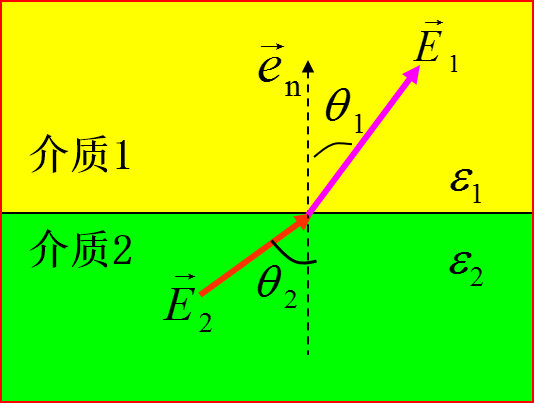
\includegraphics[keepaspectratio]{pics/场矢量折射关系}
	\caption{场矢量折射关系}
	\label{fig:fieldrefraction}
\end{figure}
$${{\tan {\theta _1}} \over {\tan {\theta _2}}} = {{{E_{{\rm{1t}}}}/{E_{{\rm{1n}}}}} \over {{E_{{\rm{2t}}}}/{E_{{\rm{2n}}}}}} = {{{\varepsilon _{\rm{1}}}/{D_{{\rm{1n}}}}} \over {{\varepsilon _{\rm{2}}}/{D_{{\rm{2n}}}}}} = {{{\varepsilon _1}} \over {{\varepsilon _2}}}$$


\section{导体表面的边界条件}
在静电平衡的情况下,导体内部的电场为0,则导体表面的边界条件为:
$$\left\{
\begin{aligned}
\vec{e}_n \times \vec{E} = 0 \\
\vec{e}_n \cdot \vec{D} = \rho_S
\end{aligned}
\right.$$

\section{电位函数}
\subsection*{电位函数}
静电场可以用一个标量函数的梯度来表示,标量函数$\phi$称为静电场的标量电位或简称电位。
$$\nabla \times \vec{E} = 0 \Rightarrow \vec{E} = -\nabla\phi$$

\subsection*{电位}
连续体分布电荷电位:
$$\phi(\vec{r}) = \frac{1}{4\pi\varepsilon} \int_V \frac{\rho(\overrightarrow{r}')}{R}\mathrm{d}V' + C$$
其中,$C$为积分操作时产生的常数。

面电荷电位:
$$\phi(\vec{r}) = \frac{1}{4\pi\varepsilon} \int_S \frac{\rho_S(\overrightarrow{r}')}{R}\mathrm{d}S' + C$$

线电荷电位:
$$\phi(\vec{r}) = \frac{1}{4\pi\varepsilon} \int_l \frac{\rho_l(\overrightarrow{r}')}{R}\mathrm{d}l' + C$$

点电荷电位:
$$\phi(\vec{r}) = \frac{1}{4\pi\varepsilon R} + C$$

\subsection*{电位差}
电场力做功(将单位正电荷从$P$移向$Q$)等于$P$、$Q$两点之间的电位差:
$$\int_P^Q E  \cdot {\rm{d}}\vec l =  - \int_P^Q {{\rm{d}}\phi }  = \phi (P) - \phi (Q)$$

\section{电位的微分方程(泊松与拉普拉斯方程)}
在均匀介质中,有泊松方程:
$$\nabla^2 \phi = -\frac{\rho}{\varepsilon}$$
在无源区域,因为$\rho = 0$,所以有:
$$\nabla^2 \phi = 0$$

\section{静电位的边界条件}
设$P_1$和$P_2$是介质分界面两侧紧贴界面的相邻两点,其电位分别为$\phi_1$和$\phi_2$。当两点间距离$\Delta l \to 0$时,$\phi_1 = \phi_2$。

$$\left\{
\begin{gathered}
\vec{e}_n \cdot (\vec{D_1} - \vec{D_2}) = \rho_S \\
\vec{D} = -\varepsilon\nabla\phi
\end{gathered}
\right. \Rightarrow {\varepsilon _2}{{\partial {\phi _2}} \over {\partial n}} - {\varepsilon _1}{{\partial {\phi _1}} \over {\partial n}} = {\rho _S}$$

若介质分界面上无自由电荷,即$\rho_S = 0$,则:
$${\varepsilon _2}{{\partial {\phi _2}} \over {\partial n}} = {\varepsilon _1}{{\partial {\phi _1}} \over {\partial n}}$$

导体表面上电位的边界条件($\phi$为常数):$$\varepsilon {{\partial \phi } \over {\partial n}} =  - {\rho _S}$$

\section{电容}
孤立导体的电容定义为所带电量$q$与其电位$\phi$的比值,即
$$C = \frac{q}{\phi}$$
电容的大小只与导体系统的几何尺寸、形状和及周围电介质的特性参数有关,而与导体的带电量和电位无关。

\subsection*{计算电容的一般方法}
\begin{enumerate}
	\item 假定两导体上分别带电荷$+q$和$-q$;
	\item 计算两导体间的电场强度$E$;
	\item 由由$U = \int^2_1\vec{E}\cdot\mathrm{d}\vec{l}$,求出导体间的电位差;
	\item 用比值法$C = \frac{q}{U}$求解电容。
\end{enumerate}

\section{静电场的能量和能量密度}
\subsection*{静电场能量}
$${W_{\rm{e}}} = {1 \over 2}q\phi $$
$${\rm{d}}{W_{\rm{e}}} = {1 \over 2}\rho \phi {\rm{d}}V$$
体分布电荷的电场能量:
$${W_{\rm{e}}} = {1 \over 2}\int_V {\rho \phi {\rm{d}}V} $$
面分布电荷的电场能量:
$${W_{\rm{e}}} = {1 \over 2}\int_S {{\rho _S}\phi {\rm{d}}S} $$

\subsection*{静电场的能量密度}
电场能量密度:
$${w_{\rm{e}}} = {1 \over 2}\vec D \cdot \vec E$$

静电场的总能量:
$${W_{\rm{e}}} = {1 \over 2}\int_V {\vec D \cdot \vec E{\rm{d}}V} $$

对于线性、各向同性介质,则有:
$${w_{\rm{e}}} = {1 \over 2}\vec D \cdot \vec E = {1 \over 2}\varepsilon \vec E \cdot \vec E = {1 \over 2}\varepsilon {E^2}$$
$${W_{\rm{e}}} = {1 \over 2}\int_V {\vec D \cdot \vec E{\rm{d}}V}  = {1 \over 2}\int_V {\varepsilon \vec E \cdot \vec E{\rm{d}}V}  = {1 \over 2}\int_V {\varepsilon {E^2}{\rm{d}}V} $$

推证:
$$W_e = {1 \over 2}\oint_S {\phi \vec D \cdot {\rm{d}}\vec S + } {1 \over 2}\int_V {\vec E \cdot \vec D{\rm{d}}V} $$

\section{恒定电场基本方程及边界条件}
\subsection*{恒定电场基本方程}
微分形式:
$$\left\{
\begin{aligned}
	\nabla \cdot \vec{J} = 0 \\
	\nabla\times\vec{E} = 0
\end{aligned}
 \right.$$

积分形式:
$$\left\{
\begin{aligned}
	\oint_S\vec{J}\cdot\mathrm{d}\vec{S} = 0 \\
	\oint_C\vec{E}\cdot\mathrm{d}\vec{l} = 0
\end{aligned}
\right.$$

线性各向同性导电媒质的本构关系:
$$\vec{J} = \sigma\vec{E}$$

若媒质是均匀的,则:
$$\nabla  \cdot {\vec J} = \nabla  \cdot (\sigma \vec E) = \sigma \nabla  \cdot \vec E = 0 \Rightarrow \nabla\cdot\vec{E} = 0$$

恒定电场的电位函数:
$$\nabla  \times {\vec E} = 0 \Rightarrow \vec E =  - \nabla \phi $$
$$\nabla  \cdot {\vec J} = 0 \Rightarrow \nabla  \cdot (\sigma \nabla \phi ) = 0\Rightarrow{\nabla ^2}\phi = 0$$

\subsection*{恒定电场的边界条件}
场矢量的边界条件:
$$\oint_S {{\vec J}}  \cdot {\rm{d}}{\vec S} = 0 \Rightarrow {\vec e_{\rm{n}}} \cdot ({{\vec J}_1} - {{\vec J}_2}) = 0 \Rightarrow {J_{1{\rm{n}}}} = {J_{{\rm{2n}}}}$$
$$\oint_C {{\kern 1pt} {\vec E}}  \cdot {\rm{d}}{\vec l} = 0 \Rightarrow {\vec e_{\rm{n}}} \times ({{\vec E}_1} - {{\vec E}_2}) = 0 \Rightarrow {E_{{\rm{1t}}}} = {E_{{\rm{2t}}}}$$

场矢量的折射关系,图\ref{fig:steadyelecfieldfraction}:
\begin{figure}[h]
	\centering
	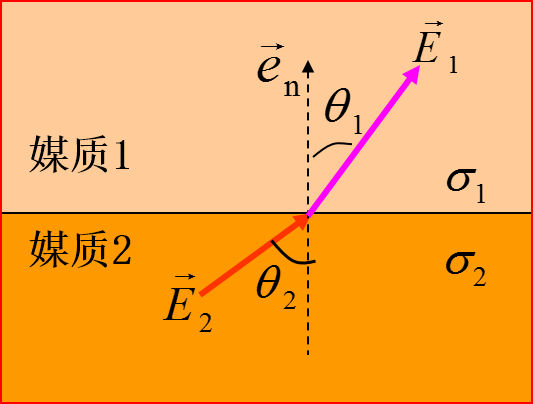
\includegraphics[keepaspectratio]{pics/恒定电场的场矢量折射关系}
	\caption{恒定电场的场矢量折射关系}
	\label{fig:steadyelecfieldfraction}
\end{figure}

$${{\tan {\theta _1}} \over {\tan {\theta _2}}} = {{{E_{{\rm{1t}}}}/{E_{{\rm{1n}}}}} \over {{E_{{\rm{2t}}}}/{E_{{\rm{2n}}}}}} = {{{\sigma _{\rm{1}}}/{J_{{\rm{1n}}}}} \over {{\sigma _{\rm{2}}}/{J_{{\rm{2n}}}}}} = {{{\sigma _1}} \over {{\sigma _2}}}$$

导电媒质分界面上的电荷面密度:
$$ \rho_S = \overrightarrow{e_n} \cdot (\vec{D_1} - \vec{D_2}) = \overrightarrow{e_n}\cdot (\frac{\varepsilon_1}{\sigma_1}\vec{J_1} - \frac{\varepsilon_2}{\sigma_2}\vec{J_2}) = (\frac{\varepsilon_1}{\sigma_1} - \frac{\varepsilon_2}{\sigma_2})J_n $$

电位的边界条件:
$${\phi _1} = {\phi _2},\quad {\sigma _1}{{\partial {\phi _1}} \over {\partial n}} = {\sigma _2}{{\partial {\phi _2}} \over {\partial n}}$$

\textbf{注:}恒定电场同时存在于导体内部和外部,在导体表面上的电场既有法向分量又有切向分量,电场并不垂直于导体表面,因而导体表面不是等位面。


\section{恒定电场与静电场的比拟(图\ref{fig:assimilation})}
PS:吐个槽,因为公式太多懒得画表格,就从PPT里面直接另存为图片的。不得不说,MathType的公式真$\cdot$吃藕。也可能是写公式的人比较懒吧。
\begin{figure}[h]
	\centering
	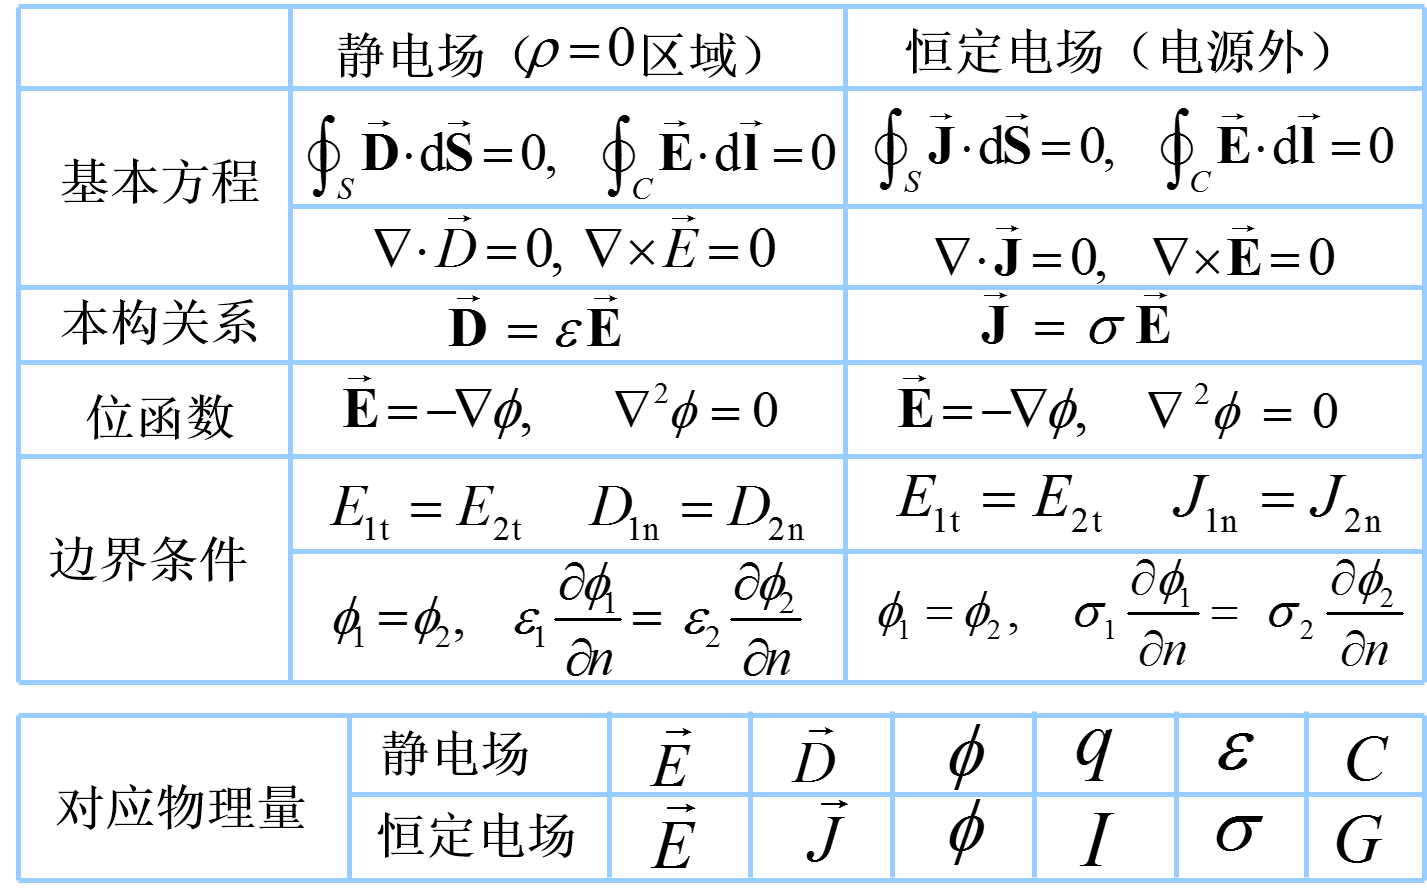
\includegraphics[width=\linewidth]{pics/恒定电场与静电场的比拟}
	\caption{恒定电场与静电场的比拟}
	\label{fig:assimilation}
\end{figure}

\section{漏电导}
漏电流与电压之比为漏电导,即:
$$G = {I \over U}$$

其倒数称为绝缘电阻,即:
$$R = {1 \over G} = {U \over I}$$

\subsection*{计算电导的方法}
\subsubsection*{法一}
\begin{enumerate}
	\item 假定两电极间的电流为$I$;
	\item 计算两电极间的电流密度矢量$\vec{J}$;
	\item 由$J = \sigma E$得到$E$;
	\item 由$U = \int^2_1\vec{E}\cdot\mathrm{d}\vec{l}$,求出两导体间的电位差。
	\item 求比值$G = \frac{I}{U}$,即得出所求电导。
\end{enumerate}

\subsubsection*{法二}
\begin{enumerate}
	\item 假定两电极间的电位差为$U$;
	\item 计算两电极间的电位分布$\varphi$;
	\item 由$\vec{E} = -\nabla\phi$得到$\vec{E}$;
	\item 由$J = \sigma E$得到$J$。
	\item 由$I = \int_S \vec{J}\cdot\mathrm{d}\vec{S}$,求出两导体间电流。
	\item 求比值$G = \frac{I}{U}$,即得出所求电导。
\end{enumerate}

\subsubsection*{法三}
经典比拟法:
$${G \over C} = {\sigma  \over \varepsilon }$$

\section{恒定磁场的基本方程和边界条件}
\subsection*{恒定磁场的基本方程}
微分形式:
\[\left\{ \begin{gathered}
\nabla  \times \vec H = \vec J \hfill \\
\nabla  \cdot \vec B = 0 \hfill \\ 
\end{gathered}  \right.\]

积分形式:
\[\left\{ \begin{gathered}
\oint_C {{\kern 1pt} \vec H}  \cdot d\vec l = \int_S {{\kern 1pt} \vec J \cdot d\vec S}  \hfill \\
\oint_S {{\kern 1pt} \vec B}  \cdot d\vec S = 0 \hfill \\ 
\end{gathered}  \right.\]

本构关系:
\[\vec B = \mu \vec H\]

\subsection*{恒定磁场的边界条件}
边界条件方程:
\[\left\{ \begin{gathered}
{{\vec e}_{\text{n}}} \cdot ({{\vec B}_1} - {{\vec B}_2}) = 0 \hfill \\
{{\vec e}_{\text{n}}} \times ({{\vec H}_1} - {{\vec H}_2}) = {{\vec J}_S} \hfill \\ 
\end{gathered}  \right.\]

若分界面上不存在面电流,即$J_S = 0$,则:
\[\left\{ \begin{gathered}
{{\vec e}_{\text{n}}} \cdot ({{\vec B}_1} - {{\vec B}_2}) = 0 \hfill \\
{{\vec e}_{\text{n}}} \times ({{\vec H}_1} - {{\vec H}_2}) = 0 \hfill \\ 
\end{gathered}  \right.\]

\section{恒定磁场的矢量磁位}
恒定磁场可以用一个矢量函数的旋度来表示:
\[\nabla  \cdot \vec B = 0 \Rightarrow \vec B = \nabla  \times \vec A\]

\subsection*{库仑规范}
与电位一样,磁矢位也不是惟一确定的,它加上任意一个标量$\varPsi$的梯度以后,仍然表示同一个磁场:
\[\vec A' = \vec A + \nabla \psi \Rightarrow \nabla  \times \vec A' = \nabla  \times \vec A + \nabla  \times (\nabla \psi ) = \nabla  \times \vec A\]
其中,$\vec{A}$为矢量磁位或称磁矢位
磁矢位的任意性是因为只规定了它的旋度,没有规定其散度造成的。为了得到确定的A,可以对A的散度加以限制,在恒定磁场中通常规定    ,并称为库仑规范。

\subsection*{磁矢位方程}
微分方程:
\[\left.
\begin{aligned}
	\vec{B} = \nabla \times \vec{A} \\
	\nabla \times \vec{B} = \mu \vec{J}
\end{aligned}
\right\} \Rightarrow \nabla \times \nabla \times \vec{A} = \mu \vec{J} \Rightarrow \nabla (\nabla \cdot \vec{A}) - \nabla^2\vec{A} = \mu \vec{J}\]

矢量泊松方程:
\[ \nabla \cdot \vec{A} = 0 \Rightarrow \nabla^2 \vec{A} = -\mu\vec{J} \]

无源区$\vec{J} = 0$时,有矢量拉普拉斯方程:
\[ \nabla^2 \vec{A} = 0 \]

\subsection*{磁矢位的表达式}
\[\nabla  \times (\frac{{\vec J(\vec r')}}
{R}{\text{)}} = \vec J(\vec r') \times \nabla (\frac{1}
{R}{\text{)}} - \frac{1}
{R}\nabla  \times \vec J(\vec r') = \vec J(\vec r') \times \nabla (\frac{1}
{R}{\text{)}} \Rightarrow \vec{A'}(\vec{r'}) = \frac{\mu}{4\pi} \int_V \frac{\vec{J'}(\vec{r'})}{R} \mathrm{d}V' \]

面电流磁矢位:
\[ \vec{A'}(\vec{r'}) = \frac{\mu}{4\pi} \int_S \frac{\vec{J'}(\vec{r'})}{R} \mathrm{d}S' \]

细线电流磁矢位:
\[ \vec{A'}(\vec{r'}) = \frac{\mu}{4\pi} \int_C \frac{\vec{J'}(\vec{r'})}{R} \mathrm{d}\vec{l'} \]

利用磁矢位计算磁通量:
\[\Phi  = \int_{{\kern 1pt} S} {\,\vec B \cdot {\text{d}}\vec S}  = \int_{{\kern 1pt} S} {\,\nabla  \times \vec A \cdot {\text{d}}\vec S}  = \oint_{{\kern 1pt} C} {{\kern 1pt} \vec A \cdot {\text{d}}\vec l} \]

磁矢位的边界条件:
\[\left.
\begin{aligned}
\oint \vec{A}\cdot\mathrm{d}\vec{l} = \int_S \vec{B}\cdot\mathrm{d}\vec{S} \Rightarrow A_{1t} = A_{2t} \\
\nabla \cdot \vec{A} = 0 \Rightarrow \oint_S\vec{A}\cdot\mathrm{d}\vec{S} = 0 \Rightarrow A_{1n} = A_{2n}
\end{aligned}
\right\} \Rightarrow \vec{A_1} = \vec{A_2} \]

\[\left.
\begin{aligned}
\vec{e_n} \times (\vec{H_1} - \vec{H_2}) = \vec{J_S} \\
\vec{H} = \nabla \times \frac{\vec{A}}{\mu}
\end{aligned}
\right\} \Rightarrow \vec{e_n} \times ( \frac{1}{\mu_1}\nabla\times\vec{A_1} -  \frac{1}{\mu_2}\nabla\times\vec{A_2}) = \vec{J_S} \]

\section{恒定磁场的标量磁位}
标量磁位或磁标位:
\[\vec H =  - \nabla {\varphi _{\text{m}}}\]
即在无传导电流(J=0)的空间中,可以引入一个标量位函数来描述磁场。

磁标位的微分方程:
\[\nabla  \cdot \vec B = 0,\vec B = {\mu _0}(\vec H + \vec M) \Rightarrow \nabla  \cdot \vec H =  - \nabla  \cdot \vec M = \frac{{{\rho _{\text{m}}}}}{{{\mu _0}}}\]
其中,等效磁荷体密度:
\[{\rho _{\text{m}}} =  - {\mu _0}\nabla  \cdot \vec M\]

将\(\vec H =  - \nabla {\varphi _{\text{m}}}\)代入\(\nabla  \cdot \vec H = \frac{{{\rho _{\text{m}}}}}{{{\mu _0}}}\)
得:
\[{\nabla ^2}{\varphi _{\text{m}}} =  - \frac{{{\rho _{\text{m}}}}}
{{{\mu _0}}}\]

在线性、各向同性的均匀媒质中:
\[{\nabla ^2}{\varphi _{\text{m}}} = 0\]

\subsection*{标量磁位的表达式}
与静电位比较,有:
\[\varphi (\vec r) = \frac{1}{4\pi\varepsilon_0}\int_V \frac{\rho (\vec r')}{R} \mathrm{d}V'\Rightarrow\varphi_\text{m}(\vec r) = \frac{1}{4\pi\mu_0}\int_V {\frac{\rho _\text{m}(\vec r')}{R}} \text{d}V'\]

\subsection*{标量磁位的边界条件}
\[\varphi_{m1} = \varphi_{m2}, \quad{\mu _1}\frac{{\partial {\varphi _{{\text{m1}}}}}}
{{\partial n}} = {\mu _2}\frac{{\partial {\varphi _{{\text{m2}}}}}}
{{\partial n}}\]
或:
\[\varphi_{m1} = \varphi_{m2}, \quad\frac{{\partial {\varphi _{m2}}}}
{{\partial n}} - \frac{{\partial {\varphi _{{\text{m1}}}}}}
{{\partial n}} =  - \frac{{{\rho _{{\text{m}}S}}}}
{{{\mu _0}}}\]
其中,有等效磁荷面密度:
\[{\rho _{{\text{m}}S}} =  - {\mu _0}{\vec e_{\text{n}}}\cdot({\vec M_2} - {\vec M_1})\]

\section{磁标位与静电位的比较(图\ref{fig:magneticeleccompare})}
\begin{figure}[h]
	\centering
	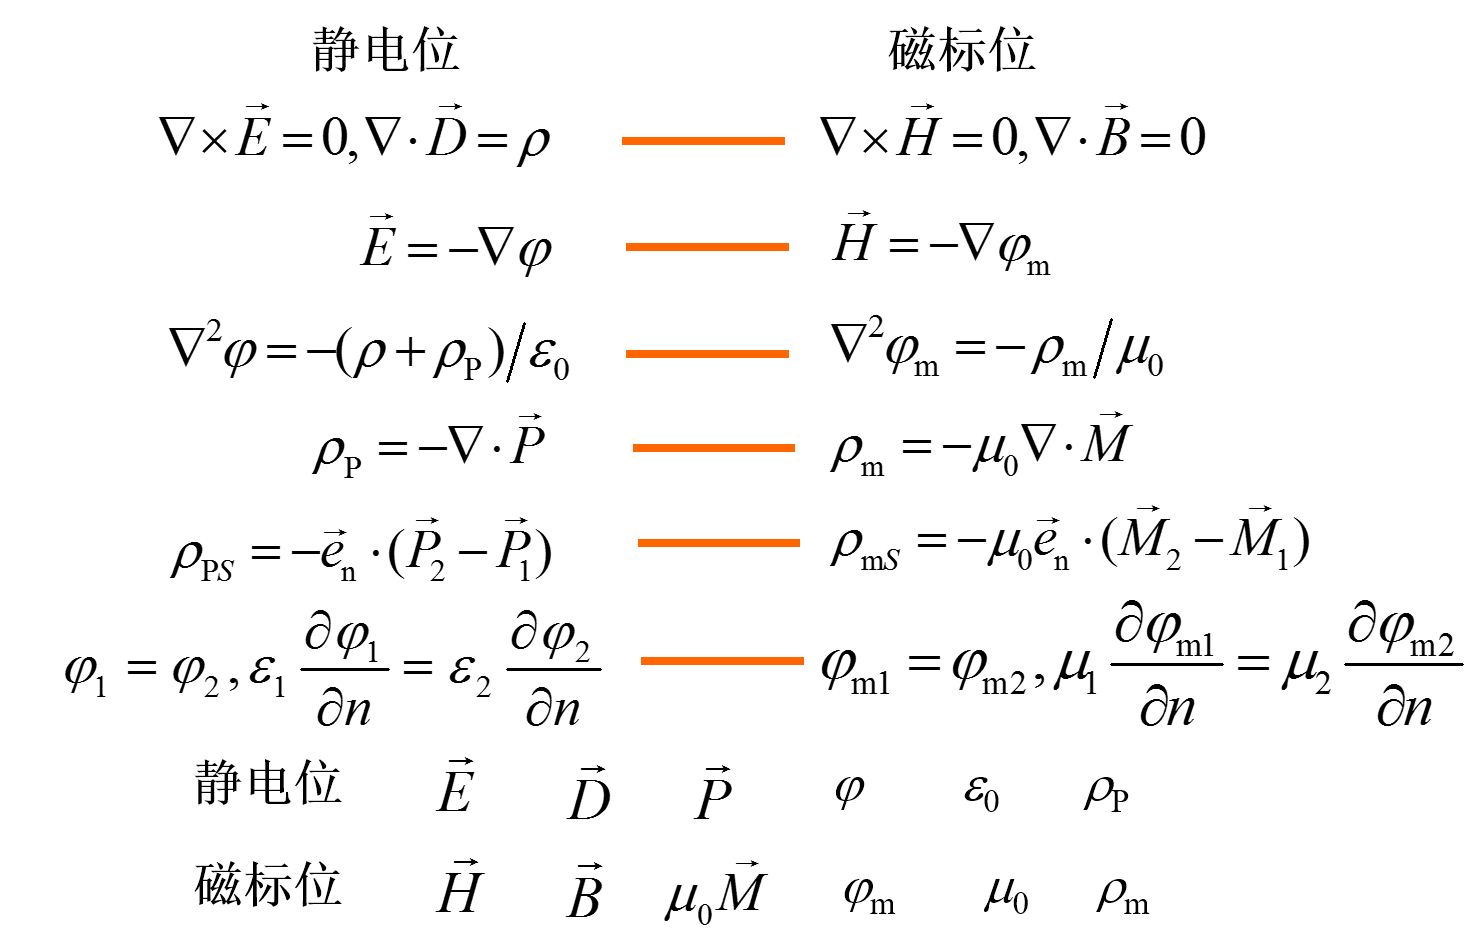
\includegraphics[width=\linewidth]{pics/磁标位与静电位的比较}
	\caption{磁标位与静电位的比较}
	\label{fig:magneticeleccompare}
\end{figure}

\section{磁通量}
单匝线圈形成的回路的磁链定义为穿过该回路的磁通量:
\[ \varPsi = \varPhi \]

多匝线圈形成的导线回路的磁链定义为所有线圈的磁通总和:
\[\Psi  = \sum_i {{\Phi _i}} \]

\section{自感}
设回路$C$中的电流为$ I $,所产生的磁场与回路$ C $交链的磁链为$ \varPsi $,则磁链$ \varPsi $与回路$ C $中的电流$ I $有正比关系,其比值
\[L = \frac{\Psi}{I}\]
称为回路 C 的自感系数,简称自感。

粗导体回路的自感:
\[ L = L_i + L_o \]
其中,$L_i = \frac{\Psi_i}{I}$为内自感,$L_o = \frac{\Psi_o}{I}$为外自感。

\section{恒定磁场的能量}



















\newpage
\begin{center}
	\textbf{未完待续:P71-P85}
\end{center}

\backmatter
% bibliography, glossary and index would go here.

\end{document}